\section{Transformaci\'on LogOdds}

Utilizar \textit{Hierarchical Agglomerative Clustering} con la distancia 
coseno y el \textit{linkage} centroide presenta al menos dos desventajas. 
Primero, la distancia coseno obliga a tener que comparar explicitamente cada
centroide con los clusters existentes. Notemos que esto implica mantener los
clusters en memoria. Por otro lado, el promedio de probabilidades no
necesariamente representa una probabilidad \cite{Pohl2007}. Esto quiere decir
que el centroide de un grupo de tractogramas no necesariamente representa un
tractograma. \\

Para solucionar estos inconvenientes proponemos transformar los tractogramas 
al espacio euclidiano utilizando la funci\'on LoggOdds. Sea $P_M$ el espacio 
de una distribuci\'on discreta para $M$ etiquetas: 

$$P_M = \left\{  p | p = (p_1,\dots p_n) \in (0,1)^M , \sum{p_i} = 1 \right\}$$

La funci\'on \textit{logit}:$P_M \rightarrow R^{M-1}$ define una transformaci\'on
entre el espacio $P_M$ y el espacio eucl\'ideo $R^{M-1}$. Dados los vectores $Q \in P^M$ y
$S \in R^{M-1}$:

$$S_i = logit(Q_i) = \frac{log(Q_i)}{log(Q_M)}$$

Para el caso de $M=2$ permite transformar la distribuci\'on Bernoulli
discreta al espacio eucl\'idio:

$$logit(p) = \frac{log(p)}{log(1-p)}$$

Trabajar en el espacio eucl\'ideo nos asegura que la suma y la multiplicaci\'on
por escalares est\'a contenido en el mismo espacio. Pohl et al. \cite{Pohl2007} 
utilizan esta propiedad para realizar operaciones lineales sobre mapas
probabil\'isticos. A su vez, demuestran que la suma y multiplicaci\'on
por escalares en el espacio eucl\'ideo poseen un significado en el espacio de la
distribuci\'on. \\

Asumiendo que cada voxel $v$ proviene de una variable aleatoria:

 $$X_v= \textrm{``La semilla est\'a conectada con el voxel v''}$$
 
Es posible aplicar la funci\'on \textit{logit} en cada voxel de los tractogramas.
El resultado es un vector donde cada coordenada se encuentra en el espacio
eucl\'ideo. Esto permite realizar operaciones lineales entre los mismos voxels
de distintos tractogramas, ya que todos provienen de una distribuci\'on
Bernoulli.\\

Nuestra segunda propuesta es cambiar la funci\'on de similitud usada durante el 
\textit{clustering}. Luego de aplicar la transformaci\'on los tractogramas
se encuentran en el espacio eucl\'ideo. Podemos entonces utilizar la m\'etrica
euclidea. Las ventajas respecto a usar la distancia coseno son varias. A 
continuaci\'on nombraremos algunas.\\



\begin{wrapfigure}{r}{0.35\textwidth}
    \begin{center}
        \vspace{-1cm}
        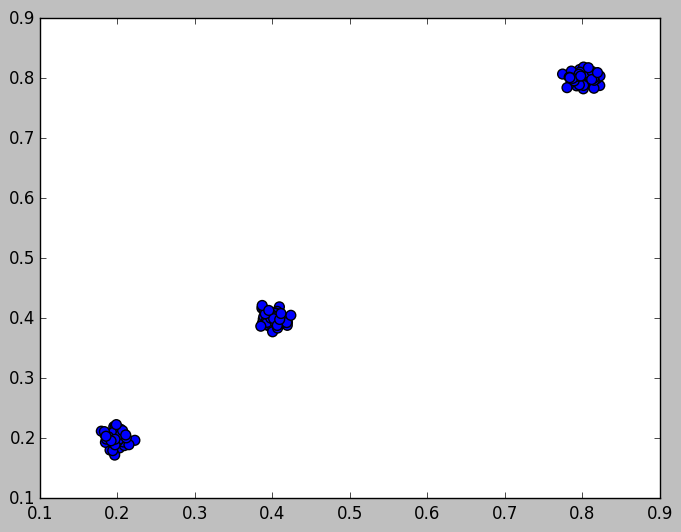
\includegraphics[width=0.35\textwidth]{img/3pop.png}
        \caption{Tres cluster colineales\-}
        \label{fig:3clusters}
    \end{center}
\end{wrapfigure}

La distancia coseno es una forma de medir correlaci\'on entre vectores. Por ello,
cuando lo que se intenta agrupar son vectores colineales el resultado es aleatorio.
Por ejemplo, cuando se aplica el procedimiento sobre los puntos de la Figura
\ref{fig:3clusters} el resultado del clustering es la Figura \ref{fig:3moreno}.
Usando LogOdds y la m\'etrica euclidiana se consigue el \textit{clustering} de 
la Figura \ref{fig:3logit}.\\

\vspace{1.5cm}

\begin{figure}[h!]

\centering                                                                                                          
\begin{minipage}[h]{0.8\textwidth}
    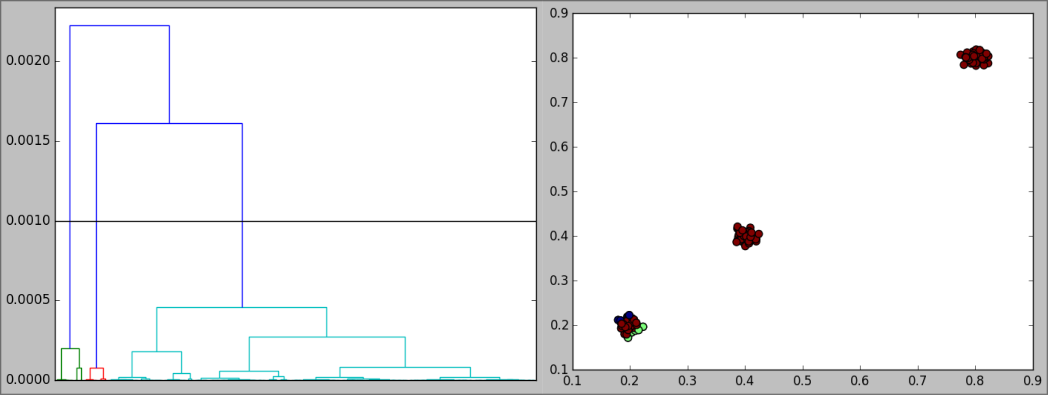
\includegraphics[width=\textwidth]{img/3pop_moreno.png}
    \caption{Clustering resultado de utilizar el m\'etodo Moreno}
    \label{fig:3moreno}
\end{minipage} ~

\end{figure}  

\begin{figure}[h!]

\centering
\begin{minipage}[h]{0.8\textwidth}
    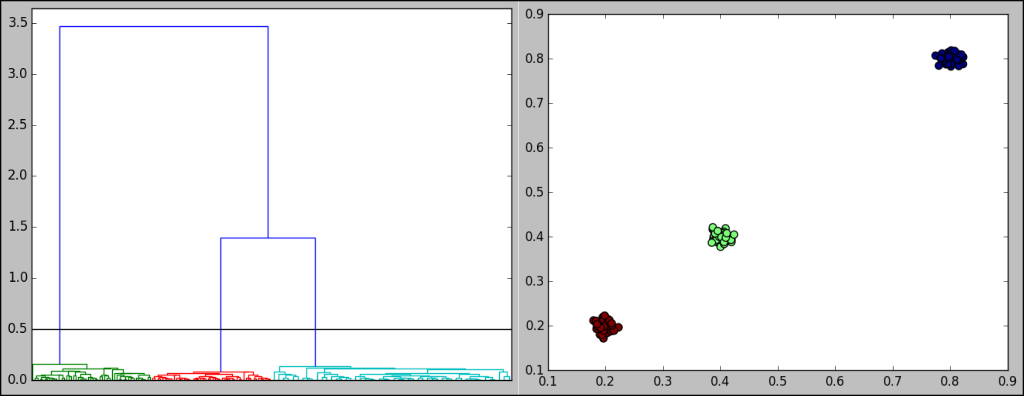
\includegraphics[width=\textwidth]{img/3pop_logit.png}
    \caption{Clustering resultado de utilizar el m\'etodo logit}
    \label{fig:3logit}
\end{minipage} ~

\end{figure}  


\subsection{Similitud vs Linkage}

La Figura \ref{fig:cos_cen} muestra cuatro vectores, sus posiciones en coordenadas
polares son: 

$$ p_1 = (0.4, 45^\circ);  p_2 = (0.3, 25^\circ); p_3 = (0.4, 66^\circ); p_4 = (0.4, 4.5^\circ)$$

Podemos apreciar que al principio $d(p_2,p_3) < d(p_3,p_4) < d(p_1,p_2)$, siendo
$d(x,y)$ la distancia coseno. Sin embargo, luego de utilizar el 
\textit{linkage centroid} sucede que $d(p_1,p_c) < d(p_4,p_c)$, esto es, $p_4$
es ahora el punto que mas lejos est\'a del centroide. Si crearamos el representante
del nuevo cluster usando el \'angulo medio entre $p_2$ y $p_3$, entonces $p_4$
seguir\'ia siendo el punto mas cercano a la uni\'on. \\

\begin{figure}[h!]
                                                                                                                        
\begin{minipage}[b]{\textwidth}
    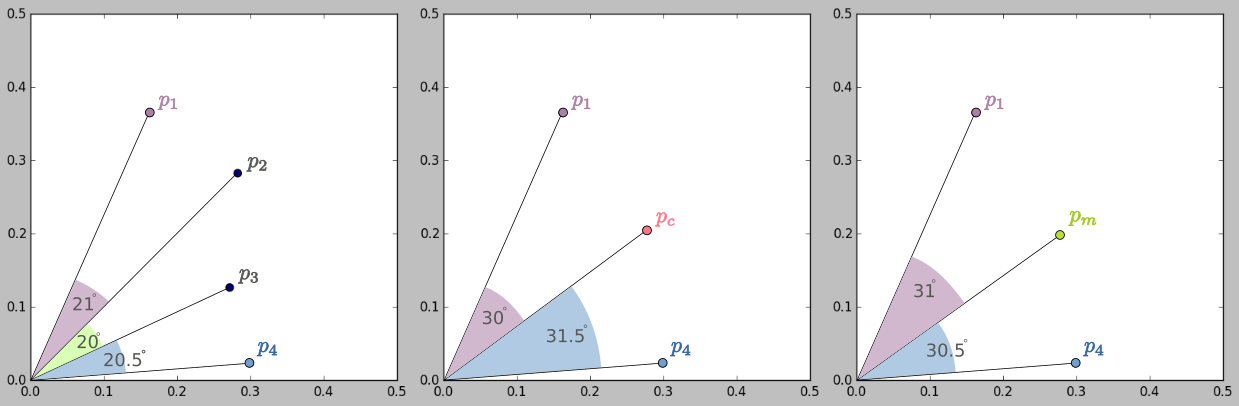
\includegraphics[width=\textwidth]{img/cosine_centroid.png}
    \caption{Contraejemplo para linkage centroide con la distancia coseno}
    \label{fig:cos_cen}
\end{minipage} ~

\end{figure}  

\textbf{Esto sucede tambi\'en con la distancia euclidea en logit}. En la Figura
\ref{fig:euc_cen}, para $l>2$, se cumple que $p_1$ est\'a m\'as cerca del centroide
que $p_4$. Recordemos que los valores dentro de los vectores luego de ser 
transformados usando LogOdds dejan de est\'ar acotados.

\begin{figure}[h!]
                                                                                                                        
\begin{minipage}[b]{\textwidth}
    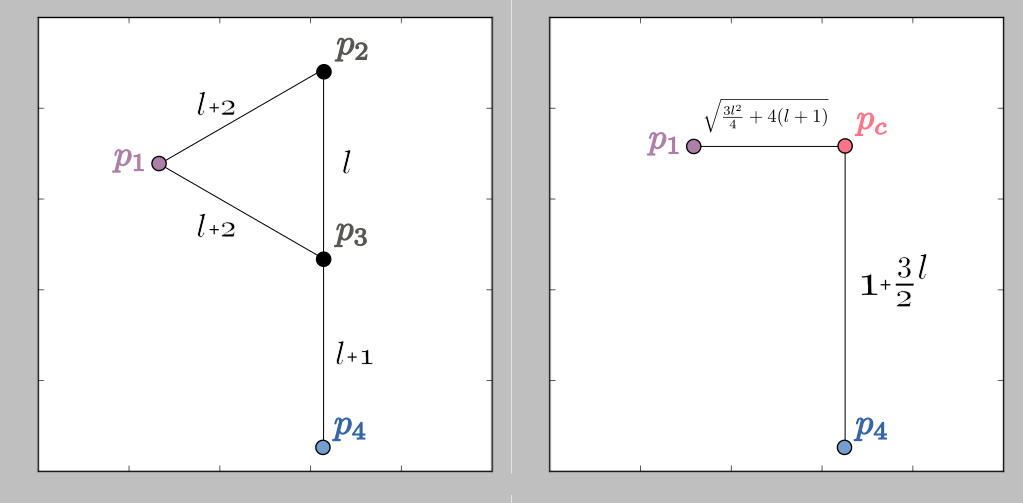
\includegraphics[width=\textwidth]{img/euclidean_centroid.png}
    \caption{Contraejemplo para linkage centroide con la distancia euclidea 
             luego de aplicar logit}
    \label{fig:euc_cen}
\end{minipage} ~

\end{figure}  

\subsection{Complejidad algor\'itmica}

Como ya explicamos, por cada iteraci\'on del algoritmo 
\textit{Agglomerative Herarchical Clustering} es necesario calcular un 
representante de la uni\'on y luego computar su distancia al resto. Sin embargo, 
al usar la m\'etrica euclideana junto con el \textit{linkage} centroide es posible
simplificar este paso. La formula de Lance y Williams permite computar las nuevas
distancias sin comparar explicitamente los clusters. Esto baja significativamente
la complejidad. Cada iteraci\'on pasa a costar $O(c^2)$ en vez de $O(c^2 m)$,
siendo $c$ la cantidad de clusters y $m$ la longitud de los mismos. La complejidad
temporal total del \textit{clustering} baja a $O(n^3)$ contra $O(n^3 m)$, siendo
$n$ la cantidad de semillas. Recordemos que en el contexto que estamos utilizando
este algoritmo $m>>n$.  

